\documentclass{report}
\usepackage[utf8]{inputenc}
\usepackage[T1]{fontenc}
\usepackage{graphicx}
\usepackage[croatian]{babel}
\graphicspath{{slike/}}
\usepackage{url}
\usepackage[hidelinks]{hyperref}

\begin{document}
\title{Osobno računalo}
\author{Nina Kafadar}
\date{17.1.2024.}
\maketitle
\tableofcontents
\listoffigures

 
\chapter{Napajanje}
Seasonic GX-850
\\ Seasonic je jedna od, ako ne i najkvalitetnija marka napajanja, napajanje je nešto skuplje od ostalih, no 10 godina garancije potvrđuje kvalitetu izrade. Napajanje je kompletno modularno što znači da se mogu koristiti samo kablovi koji su potrebni za rad računala što znači da će kablova biti manje zbog čega će biti bolje strujanje zraka te će biti manje grijanja, također radi samog izgleda računala (cable management). 850W je i više nego dovoljno za pokretanje računala koje će se koristiti za rad, te u slučaju nadogradnje računala grafičkom karticom, napajanje će biti dovoljno snažno te se neće morati mijenjati.
\\Specifikacije: 
\\Snaga: 850W
\\Temperatura rada 0 – 40°C
\begin{figure}[h]
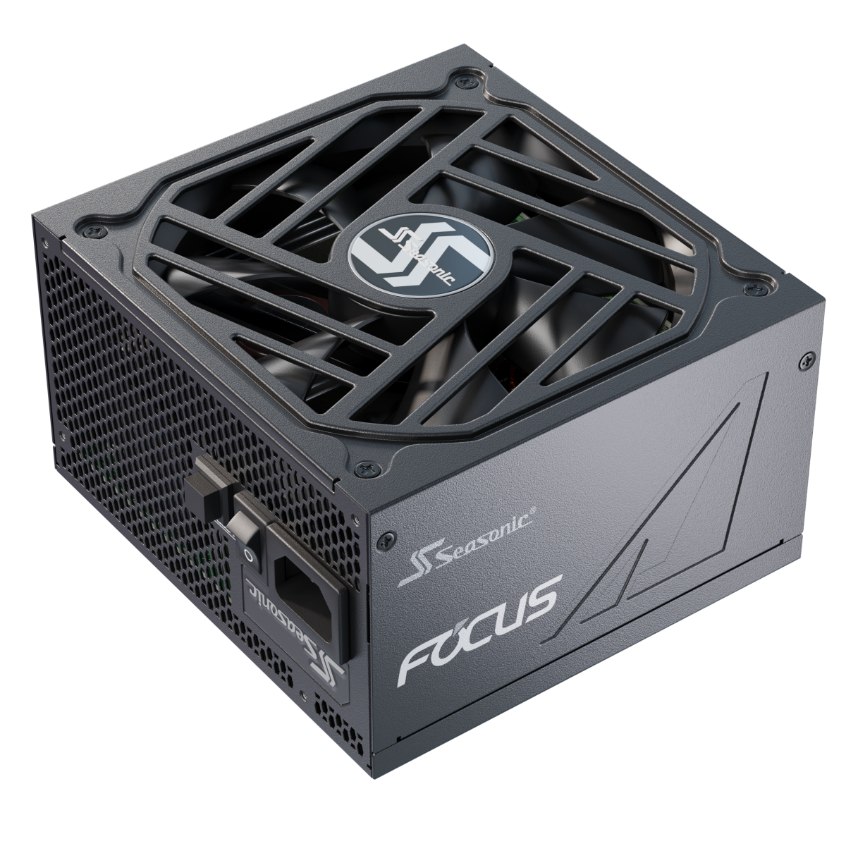
\includegraphics[width=8cm]{Napajanje.png}
\caption{Seasonic GX-850}
\end{figure}


\chapter{Matična}
Asus-z790-rog-strix-z790-a-gaming-wifi
\\ Ploča dolazi s ugrađenim hladnjacima za ključne komponente poput SSD-ova, hladnjaci za chipset itd. Sadrži sve potrebne konektore za komponente koje će se koristiti u ovom računalu, no ima mjesta i za nadogradnju ukoliko bude potrebno. Ploča također dolazi s Wi-Fi 7 antenom.
\\Specifikacije:
\\Vrsta/veličina ploče: ATX
\\Socket i chipset: Intel 1700, Intel Z790
\\Ram: 4x DDR5 DIMM, maksimalan kapacitet 192GB, maksimalna brzina 8000 MHz
\\Utori za komponente: 1x PCIe 5.0 x16, 1x PCIe 4.0 x16 (x4), 1x PCIe 3.0 x1, 1x M.2/M-Key (PCIe 4.0 x4, 22110/2280/2260/2242), 2x M.2/M-Key (PCIe 4.0 x4, 2280), 1x M.2/M-Key (PCIe 4.0 x4, 22110/2280/2260/2242), 1x M.2/M-Key (PCIe 4.0 x4/SATA, 2280/2260/2242), 1x M.2/E-Key (Intel CNVi, 2230, occupied with WiFi+BT module)
\\Vanjski utori: 1x HDMI 2.1 (iGPU), 1x DisplayPort 1.4 (iGPU), 1x USB-C 3.2 (20Gb/s), 1x USB-C 3.1 (10Gb/s), 2x USB-A 3.1 (10Gb/s), 4x USB-A 3.0 (5Gb/s), 4x USB-A 2.0 (480Mb/s), 1x 2.5GBase-T (Intel I226-V), 2x jack, 1x Toslink, 2x antenna connector RP-SMA proprietary
\\Dodatno: Vanjsko flashbackanje BIOS-a  pomoću USB-a i vanjski gumb za brisanje CMOS-a
\\Napajanje ploče: 1x 24 pin
\begin{figure}[h]
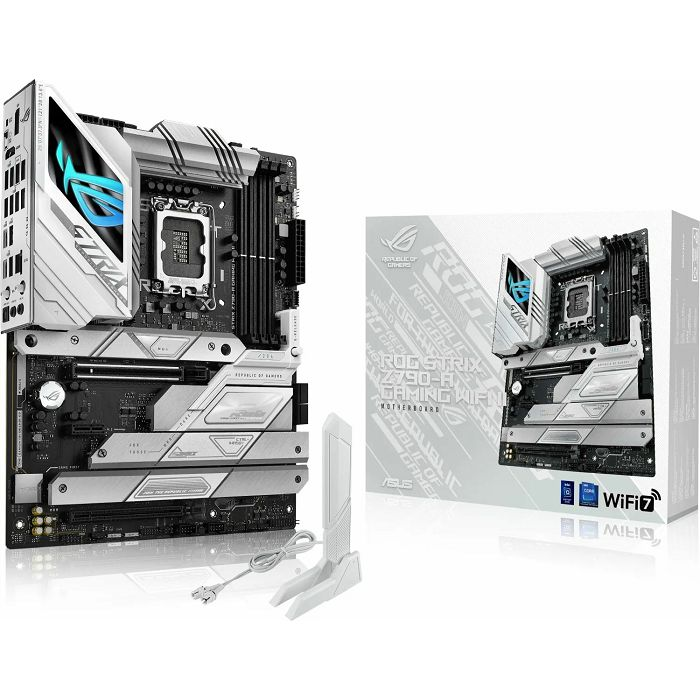
\includegraphics[width=8cm]{Matična.jpg}
\caption{Asus-z790-rog-strix-z790-a-gaming-wifi}
\end{figure}


\chapter{Procesor}
 Intel core i7 14700k
\\Intel procesori su vrlo kvalitetni i brzi procesori koji su ujedino i jako efikasni. Također procesori dolaze s integriranom grafikom što je idealno za poslovne potrebe ukoliko ne želimo koristiti dodatnu grafičku karticu. Velik broj jezgri i vritualnih jezgri vrlo je bitan za manja vremena kompajliranja koda, otvaranja programa i slično.
\\Specifikacije:
\\Jezgri: 20 (8 performansnih jezgri i 12 učinkovitih jezgri)
\\Performansne: Bazna frekvencija 3.4 GHz, turbo 5.5 GHz
\\Učinkovite: Bazna frekvencija 2.5 GHz, turbo 4.3 GHz
\\Vritualnih jezgri: 28
\\Cache: 33MB Intel Smart Cache
\\Snaga: Bazna 125W, Turbo 253W
\\Memorija: Maksimalan kapacitet 192GB, DDR5 do 5600 MT/s, DDR4 do 3200 MT/s, maksimalno 2 kanala, maksimalan bandwidth 89.6 GB/s
\\GPU: Intel UHD Graphics 770, frekvencija 300MHz, maksimalna rezolucija HDMI 4090 x 2160 @60Hz, maksimalna rezolucija DP (display port) 7680 x 4320 @60Hz, DirectX podrška za verziju 12, podrška za do 4 ekrana.
\begin{figure}[h]
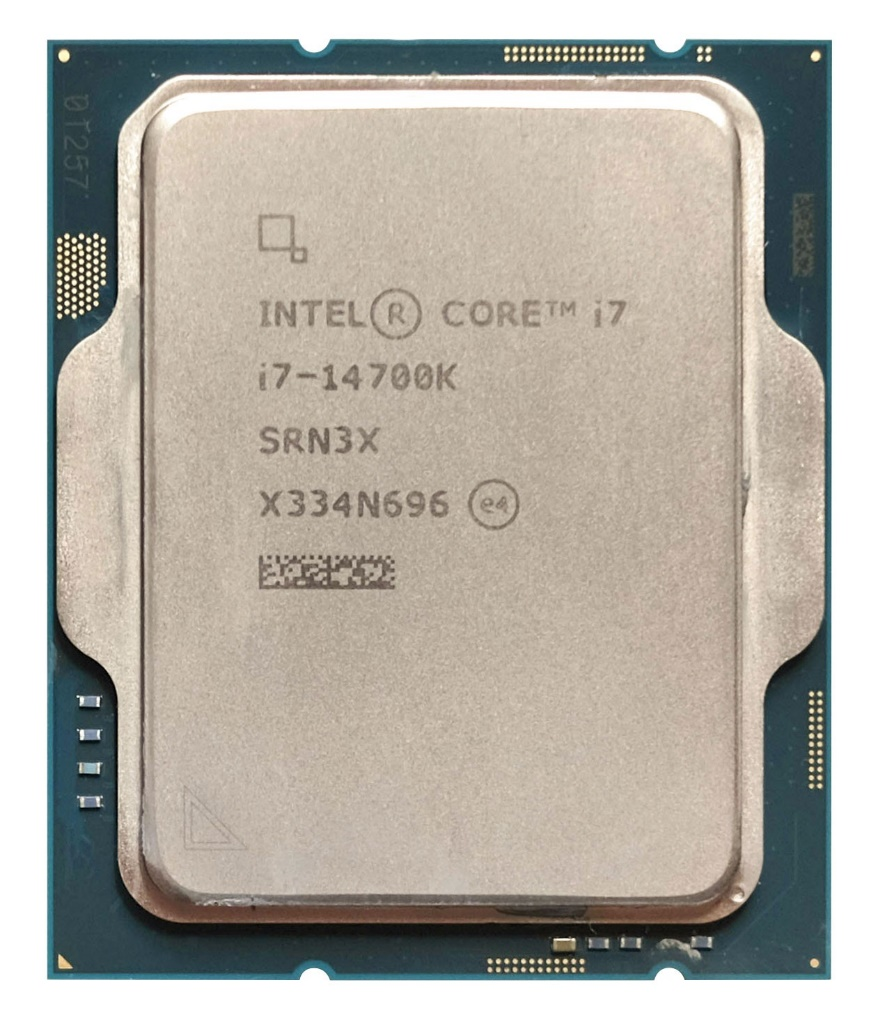
\includegraphics[width=8cm]{Procesor.jpg}
\caption{Intel core i7 14700k}
\end{figure}


\chapter{Hladnjak za procesor}
Noctua nh u12a chromax black
\\Noctua je vrlo popularan brand za procesorske hladnjake, ovaj hladnjak dolazi s 2 ventilatora koja mogu biti stavljena po potrebi, također hladnjak je velikih dimenzija što pomaže pri rasprostranjivanju topline. Veličina hladnjaka također znači bolje hlađenje procesora. Hadnjak, osim svojstva kvalitetnog hlađenja jako lijepo izgleda te je u crnoj boji.
\\Specifikacije:
\\Dimenzije s ventilatorima (ŠxVxD) 125x158x112mm
\\Dimenzije bez ventilatora (ŠxVxD) 125x158x58mm
\\4-pin PWM konektor
\begin{figure}[h]
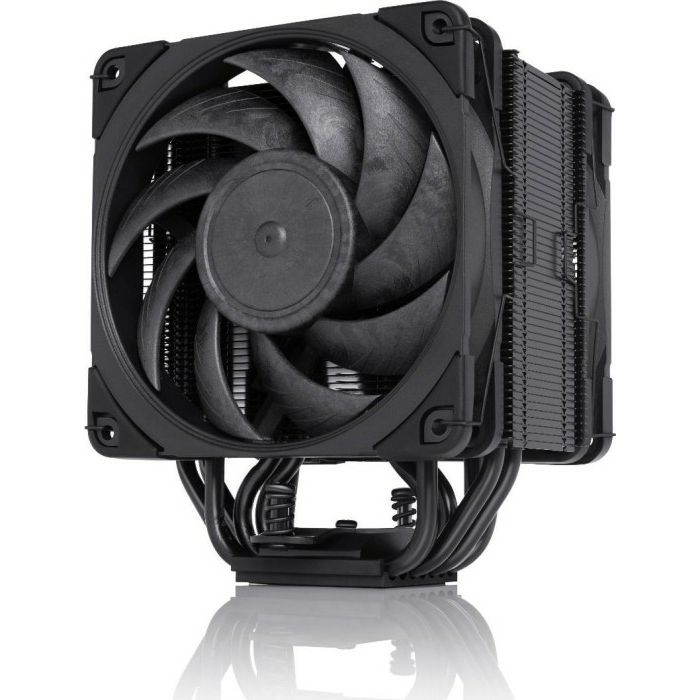
\includegraphics[width=8cm]{Hladnjak za procesor.jpg}
\caption{Noctua nh u12a chromax black}
\end{figure}


\chapter{Radna memorija}
G.Skill Trident Z5 Black (2x32) 6000MHz
\\G.Skill je vrlo kvalitetan brand radne memorije te najčešće koriste Samsungove čipove. Ovi rami također dolaze s ugrađenim hladnjakom što je vrlo dobro s obzirom na brzinu i količinu čipova koji se mogu dosta zagrijati tijekom zahtjevnijih operacija. Za obavljanje poslova gdje je potrebno imati puno otvorenih programa i podosta browser tabova ,potrebno je imati i dosta veliki kapacitet radne memorije. 64GB u dvije pločice je i više nego dovoljno za sve potrebne radnje, te ostavlja prostora za nadogradnju s obzirom da matična ploča i processor podržavaju veći kapacitet.
\\Specifikacije:
\\Količina: 64GB (2x32GB)
\\Tip: DDR5 DIMM 288 Pin
\\Takt: 6000MHz
\\Latencija: CAS CL30, tRCD 40, tPR 40, tRAS 96
\\Voltaža: 1.4V
\\Visina: 43.5mm
\\Intel XMP 3.0
\begin{figure}[h]
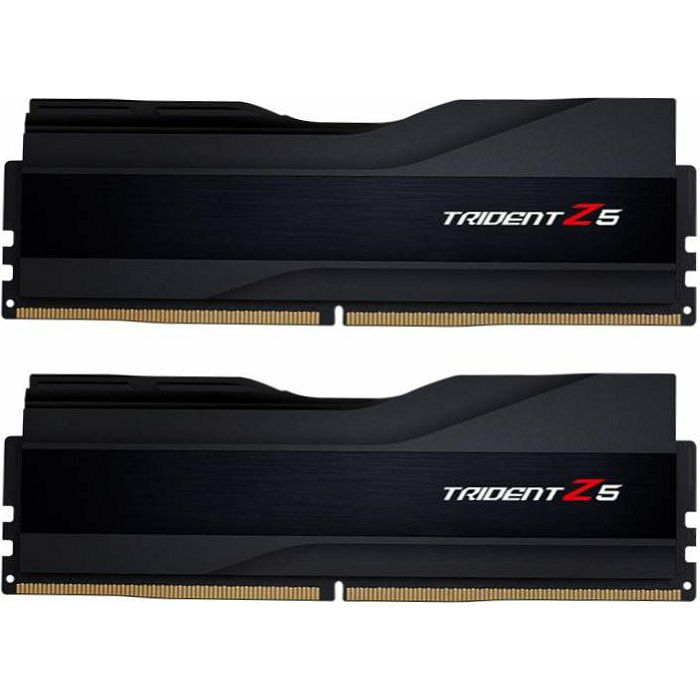
\includegraphics[width=8cm]{Radna memorija.jpg}
\caption{G.Skill Trident Z5 Black (2x32) 6000MHz}
\end{figure}



\chapter{Pohrana}
Samsung 990 PRO M.2 1TB
\\ Samsung se vrlo brzo probio i postao je broj jedan u računalnoj dugotrajnoj pohrani podataka. Također Samsungovi M.2 SSD-ovi imaju jako velike brzina čitanja i zapisivanja uz veliku dugovječnost. Velike brzine čitanja i zapisivanja su vrlo bitne kako bi se što manje čekalo na učitavanje svih radnji, od učitavanja programa tijekom pokretanja, do učitavanja slika, videa i slično. 1TB je sasvim dovoljno prostora za sve programe ali i pohranu nekih osobnih stvari.
\\Specifikacije:
\\Tip: M.2
\\PCIe: 4.0 x4
\\Čitanje: 7450 MB/s
\\Zapisivanje: 6900 MB/s
\\Potrošnja: 7.8W(maksimum), 5.4W (operacionalno), 0.05W (idle), 0.005W (način spavanja)
\begin{figure}[h]
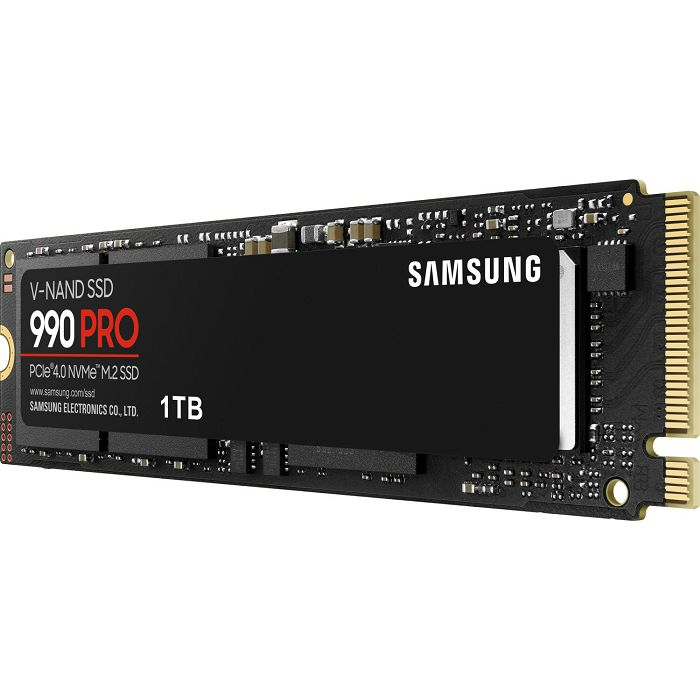
\includegraphics[width=8cm]{Pohrana.jpg}
\caption{Samsung 990 PRO M.2 1TB}
\end{figure}


\chapter{Kućište}
Fractal Design North Charcoal Black TG
\\Fractal Design proizvodi jako kvalitetna kućišta, stoga dugo traju. Dugo trajanje u smislu kućišta znači da se gumbići i utori na kućištu neće samo tako potrgati. Također, poznati su po vrlo dobrom strujanju zraka te imaju velik broj mjesta za postavljanje komponenti za pohranu koje su skrivene od oka čak i kada kućište ima stakleni bočni panel. Kućište jako lijepo izgleda što je također veliki plus.
\\Specifikacije:
7 utora za proširenje, 2x 3.5”, 2x 2.5” SSD, 2x USB 3.0, 1x USB 3.1 Gen2 Type-c, 1x Audio, 1x Mikrofon, 
\\mogućnost ventilatora: 
prednji 2x 120 ili 2x 140 mm PWM
gronji 2x 120 ili 140 mm
stražnji: 1x 120mm
\\Podržani formati ploča: ATX, mATX, ITX
\\Podrška za hladnjake do 145mm visine, podrška za GPU dužine do 355mm, podrška za vodena hlađenja
\begin{figure}[h]
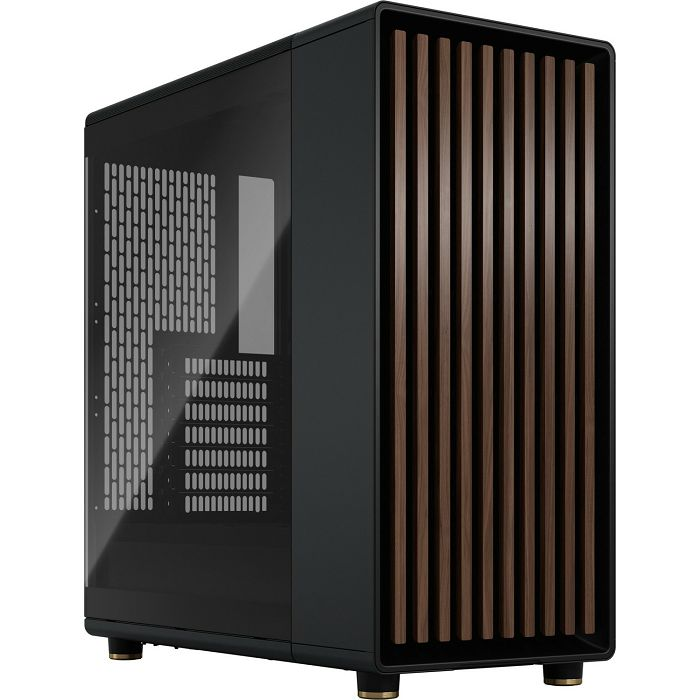
\includegraphics[width=8cm]{Kućište.jpg}
\caption{Fractal Design North Charcoal Black TG}
\end{figure}


\chapter{Monitor}
Samsung Odyssey CRG9
\\Ovaj monitor odabran je radi veličine ekrana te zato što je najjeftiniji monitor tog tipa. Radi ultra širokog formata slike, na ekran istovremeno, bez ikakvih problema mogu stati čak 3 prozora što dosta olakšava programiranje. Tako istodobno u web programiranju možemo vidjeti samu aplikaciju, konzolu web browsera i IDE. Također QHD rezolucija znači da više stvari stane na ekran, te je ljepše za gledati u kvalitetniju sliku.
\\Specifikacije:
\\Panel: VA
\\Tehnologija: QLED
\\Rezolucija: 5120x1440 (veličina dva 27” QHD monitora)
\\Format slike: 32:9 (ultrawide)
\\Zakrivljenost ekrana: 1800R
\\Vidljivi kut: 170° visina i 178° širina
\\Maksimalna svjetlina: 1000 CD/m2
\\Podrška boje: Maks. 1.07 milijardi boja
\\Osvježenje ekrana (Koliko puta se slika osvježi u jednoj sekundi): Maks. 120Hz
\\Utori: HDMI 2.0, USB x4
\\Temperatura rada: 10~40°C
\\Ostalo:
AMD Radeon FreeSync: smanjenje prekida i trešnje slike, podrška za HDR sadržajem, smanjeno ulazno kašnjenje i kompenzacija niskog broja prikazanih slika
\begin{figure}[h]
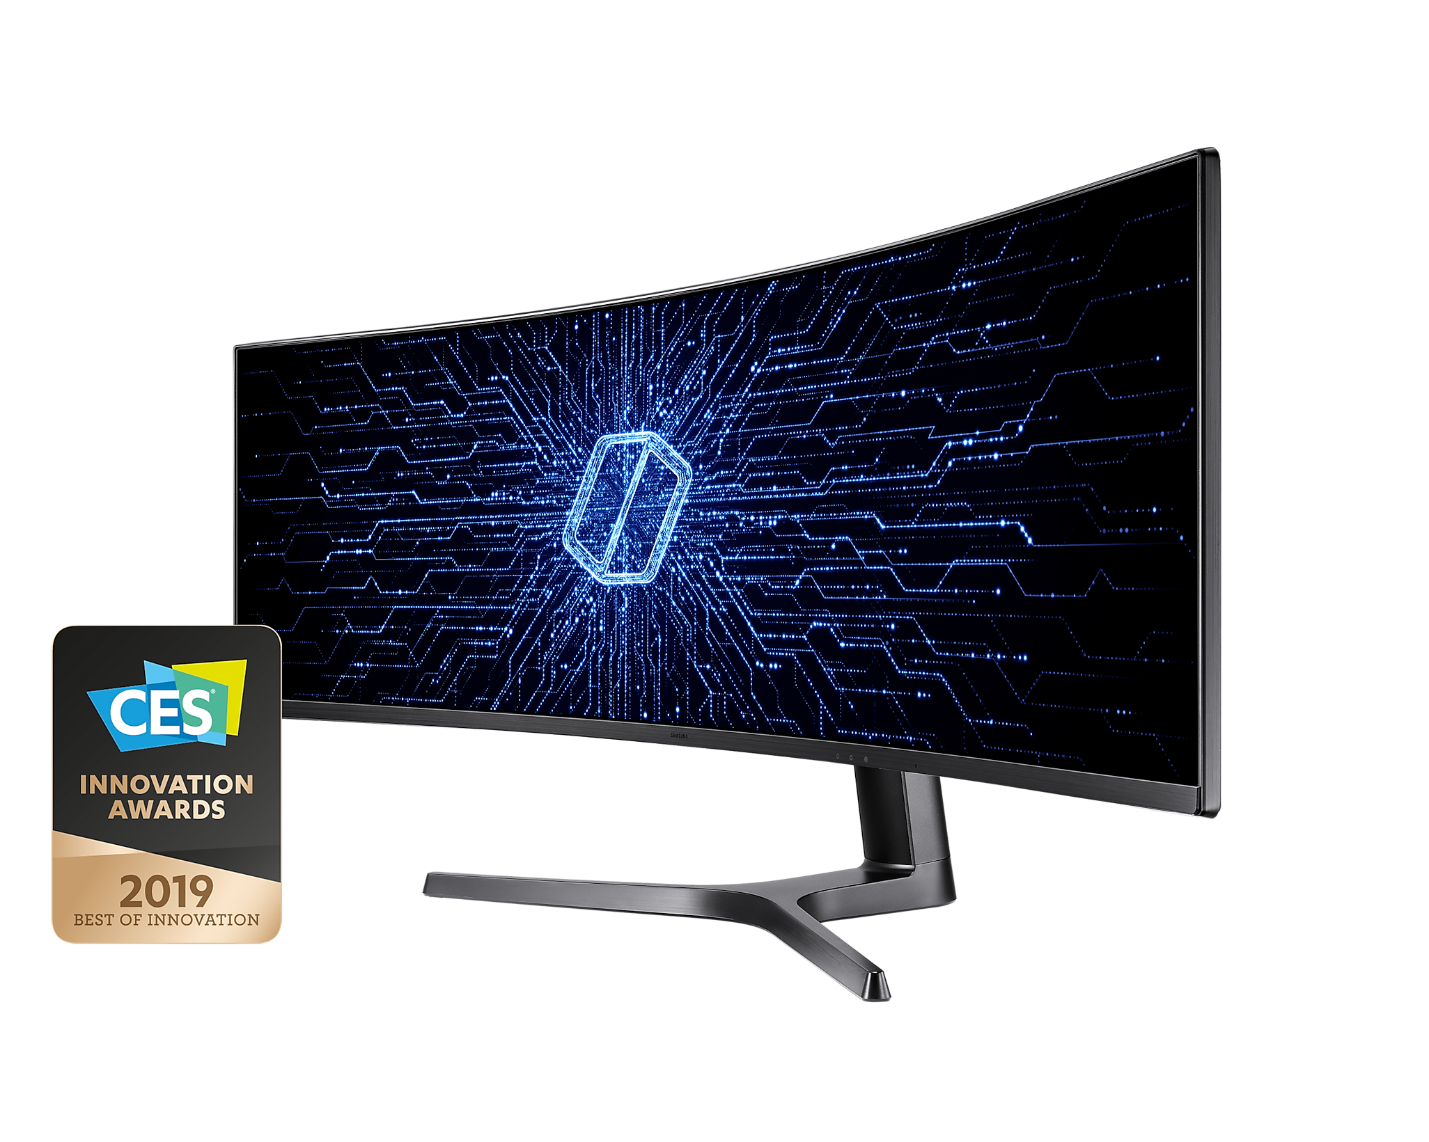
\includegraphics[width=8cm]{Monitor.png}
\caption{Samsung Odyssey CRG9}
\end{figure}

\chapter{Miš}
 Logitech Mx Master 3s
\\Srednji Scroll koristi infinity scroll tehnologiju što znači da se može scrollati kroz 1000 linija po sekundi. 1 minuta punjenja miša daje 3 sata korištenja, dok na punoj bateriji daje 70 dana rada. Koristi Bluetooth za povezivost koja je omogućena pomoću Logi Bolt USB recievera koji se dobije u pakiranju s mišem. Miš podržava više operativnih sustava, također na dnu miša nalazi se gumb pomoću kojeg možemo lagano prebaciti miša na drugi uređaj (do 3 uređaja). Na mišu se također nalazi horizontalni scroll, gumb za akcije na odmorištu za prst i naprijed/nazad gumbovi koji su na odličnoj poziciji te je jako lagano za raditi s njima. Miš je napravljen od kvalitetnih materijala, S u nazivu opisuje riječ “Silent” što znači da su sve tipke jako tihe tijekom korištenja. Za potrebe ovog miša Logitech nam pruža skidanje bestplatnog upravljačkog programa Logi Options+ u kojem možemo iskonfigurirati doslovno sve na samom mišu, tako možemo zamijeniti desni za lijevi klik, možemo odrediti brzinu scrollanja glavnog ali i horizontalnog scrolla, možemo promijeniti smjer scrollanja, sve tipke možemo namjestiti željene prečace ili akcije, također sve opisano se može namjestiti posebno za svaku aplikaciju što znači da gumb za nazad na Visual Studiu možemo koristiti recimo za zatvaranje trenutno otvorenog dokumenta, dok na Visual Studio Codu može biti odlazak u prethodno otvoreni document i slično. Miš također dolazi sa Flow značajkom koju možemo namijestiti u Logi Options+ upravljačkom programu, ova značajka omogućava korištenje miša na 2 uređaja odjednom, kada dođemo do horizontalnog kraja ekrana na jednom uređaju, miš će se automatski prebaciti na drugi uređaj, tako možemo s jednog uređaja kopirati datoteke na drugi uređaj bez ikakvih problema.
\begin{figure}[h]
\includegraphics[width=8cm]{Miš.jpg}
\caption{Logitech Mx Master 3s}
\end{figure}


\chapter{Tipkovica}
Logitech MX Keys
\\Mx Keys tipkovnica je savršena tipkovnica u paru s Mx Master 3s mišem, koristi sensor za blizinu kako bi se upalilo pozadinsko osvjetljenje tipki što je tijekom dugih radnih noći lijepo za vidjeti pošto nekada znamo fulati tipke ili položaj ruku na tipkovnici. Kao i miš, ova tipkovnica je vrlo tiha ali i tipke koje imaju udubljenje u obliku kruga dodaju na udobnosti korištenja. Baterija traje vrlo dugo, tipkovnica sadrži 3 tipke koje pružaju mogućnost prebacivanja s jednog uređaja na drugi. Mx Keys dolazi s funkcijskim tipkama za smanjenje svjetline, prebacivanje pjesama, smanjivanje glasnoće, otvaranje kalkulatora, slikanje ekrana, zaključavanje uređaja i tako dalje. Sve funkcijske tipke su konfigurabilne pomoću Logi Options+ upravljačkog programa.
\\Specifikacije:
\\Baterija: Punjiva Li-Po (1500 mAh), trajanje 10 dana na punom punjenju ili 5 mjeseci s isključenim pozadinskim osvjetljenjem tipki
\\Povezivost: Bluetooth pomoću Logi Bolt USB, 3 Easy Switch tipke za povezivost s do 3 uređaja
\\Punjenje: USB C
\begin{figure}[h]
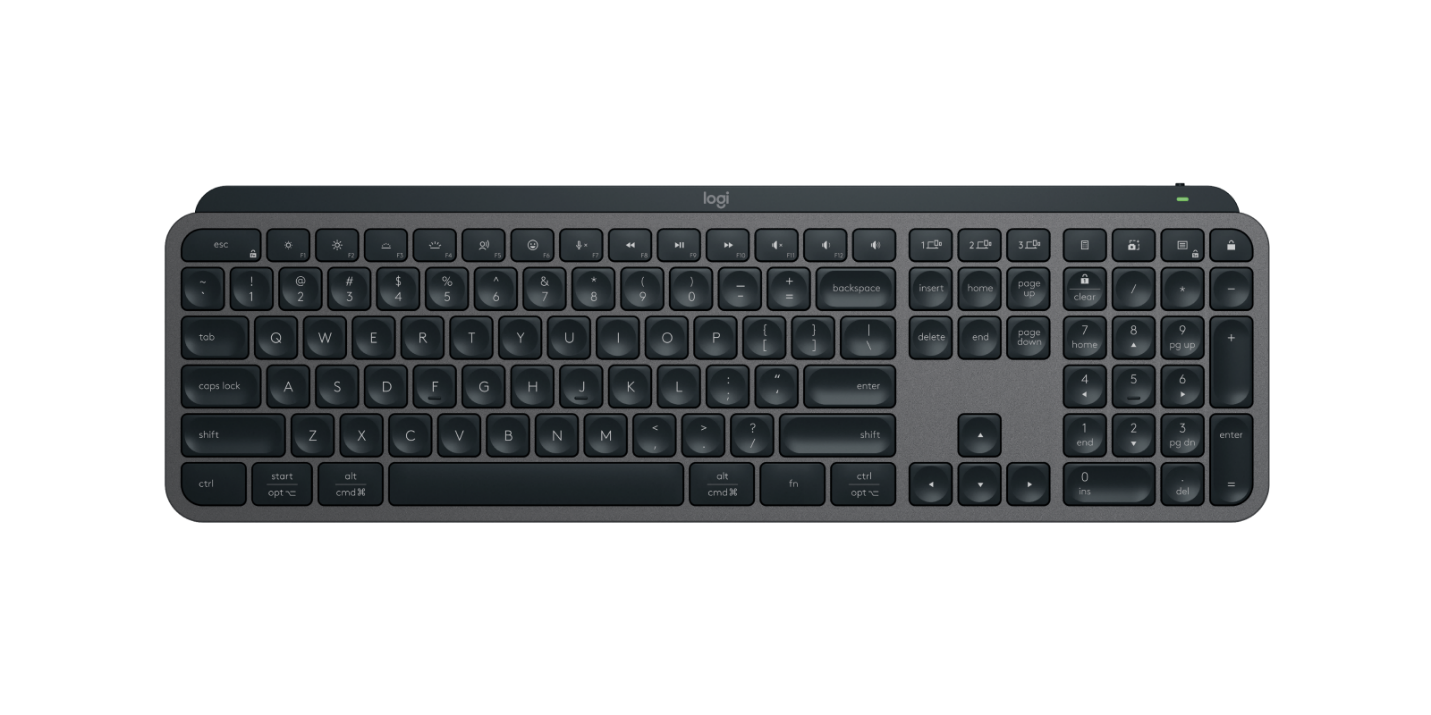
\includegraphics[width=8cm]{Tipkovnica.png}
\caption{Logitech MX Keys}
\end{figure}


\chapter{Cijena i namjena}
Svrha i ciljana upotreba ovog računala je svestrano korištenje uz određene nadogradnje, no primarno za poslovno korištenje, točnije za programiranje. Ovo računalo je vrlo skupo, no ono je složeno kako bi moglo biti korišteno 10 godina s obzirom na kvalitetu i jačinu odbranih komponenti, također može se nadograditi. Vrlo snažne komponente omogućavaju vrlo brz rad bez ikakvog štekanja, tako se prevođenje koda  u strojni kod, otvaranje mnogobrojnih programa i samo korištenje odvija vrlo brzo. Nadogradimo li ovo računalo sa grafičkom karticom, ovo računalo može pokrenuti najjače igrice. Također, ovo računalo se nadogradnjom grafičke može koristiti za video renderiranje i mnoge druge stvari.
\\Cijene: 
\\ \href{https://www.adm.hr/napajanje-seasonic-850w-focus-gx-850-full-modular-80-plus-gold-atx-/79129/product/?utm_source=nabava.net&utm_campaign=nabava.net&utm_medium=click}{Napajanje}: 173,68€ 
\\ \href{https://www.adm.hr/asus-z790-rog-strix-z790-a-gaming-wifi-ii-ddr5-intel-s1700-90mb1fn/79373/product/}{Matična}: 515,79€
\\ \href{https://www.adm.hr/intel-core-i7-14700k-34ghz-lga1700-boxed-without-cooler-bx807151470/78722/product/}{Procesor}: 536,84€
\\ \href{https://www.adm.hr/noctua-nh-u12a-chromax-black/70965/product/}{Hladnjak za procesor}: 134,74€ 
\\ \href{https://www.adm.hr/ddr5-64gb-2x32-gskill-6000mhz-trident-z5-black-cl30-f5-6000j3040g32gx2-tz/75778/product/}{Radna memorija}: 309,47€ 
\\ \href{https://www.adm.hr/samsung-ssd-1tb-990-pro-m2-pcie-40-x4-mz-v9p1t0bw-600tbw/75929/product/}{Pohrana}: 145,26€ 
\\ \href{https://www.adm.hr/fractal-design-north-charcoal-black-tg-light-tint-fd-c-nor1c-02/76085/product/}{Kućište}: 188,42€
\\ \href{https://www.mikronis.hr/Proizvod/monitor-samsung-odyssey-crg9-lc49rg90sspxen-49-dual-qhd-va-ultrawide-zakrivljeni-120hz-4ms-2x-hdmi-dp-minidp-audio-2x-usb/40472}{Monitor}: 949€
\\ \href{https://www.adm.hr/logitech-mx-master-3s-graphite-910-006559/73919/product/}{Miš}: 125,26€
\\ \href{https://team-media.hr/proizvod/logitech-mx-keys-kabellose-tastatur-graph-business-version-uk-layout-920-010250/?utm_source=nabava.net&utm_campaign=nabava.net&utm_medium=click}{Tipkovnica}: 170€
\\Ukupna cijena: 3248,47€

\end{document}